\documentclass[tikz,border=10pt]{standalone}
\usetikzlibrary{shapes}
\usetikzlibrary{arrows}
\usetikzlibrary{positioning}
\begin{document} 
%% Draws a hundred blocks random city
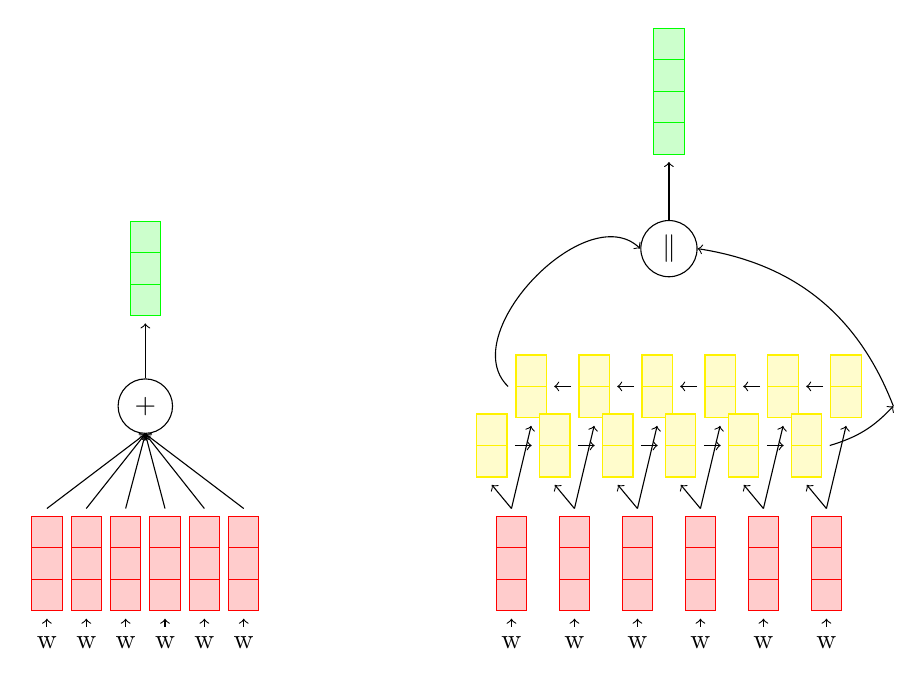
\begin{tikzpicture}[
  hid/.style 2 args={
    rectangle split,
    draw=#2,
    rectangle split parts=#1,
    fill=#2!20,
    outer sep=1mm}]

 \foreach \i [count=\step from 1] in {w, w, w, w, w, w}
    \node (i\step) at (.5*\step, -2) {\i};
  % draw embedding and hidden layers for text input
  \foreach \step in {1,...,3} {
    \node[hid={3}{red}] (e\step) at (.5*\step, -1) {};    
    \draw[->] (i\step.north) -> (e\step.south);
  }
  \foreach \step in {4,...,6} {
    \node[hid={3}{red}] (e\step) at (.5*\step, -1) {};    
    \draw[->] (i\step.north) -> (e\step.south);
  }
 
 \node[circle,draw=black] (avgpool) at (1.75, 1) {$+$};
 
  \foreach \step in {1,...,6} {
    \node[hid={3}{red}] (e\step) at (.5*\step, -1) {};    
    \draw[->] (e\step.north) -> (avgpool.south);
  }
 
 \node[hid={3}{green}] (s1) at (1.75, 2.75) {};
 \draw[->] (avgpool.north)->(s1.south);


 \foreach \i [count=\step from 8] in {w, w, w, w, w, w}
    \node (i\step) at (.8*\step, -2) {\i};
  % draw embedding and hidden layers for text input
  \foreach \step in {8,...,13} {
    \node[hid={3}{red}] (e\step) at (.8*\step, -1) {};    
    \draw[->] (i\step.north) -> (e\step.south);
  }

  \foreach \step in {8,...,13} {
    \node[hid={2}{yellow}] (h_f_\step) at (-.25 + .8 *\step, .5) {};    
    \node[hid={2}{yellow}] (h_r_\step) at (.25 + .8 *\step, 1.25) {};    
    \draw[->] (e\step.north) -> (h_f_\step.south);
    \draw[->] (e\step.north) -> (h_r_\step.south);
  }
 % \foreach[count=\i, evaluate=\i as \x using int(\i+9)] \step in {8,...,10} {
  \foreach \step/\steppp in {8/9, 9/10, 10/11, 11/12, 12/13} {
   
    \draw[->] (h_f_\step.east) -> (h_f_\steppp.west);
    \draw[->] (h_r_\steppp.west) -> (h_r_\step.east);
  }
 
\node[circle,draw=black] (concat) at (8.4, 3) {$\Vert$};
\coordinate (g) at (11.25, 1);
\path[->] (h_r_8.west) edge[bend left=90] (concat.west);
\path[->] (h_f_13.east) edge[bend right=15] (g) 
          (g) edge[bend right] (concat.east);
\node[hid={4}{green}] (s2) at (8.4, 5) {};
\path[->] (concat) edge (s2);
 
% \node[circle,draw=black] (avgpool) at (1.75, 1) {$+$};
% 
%  \foreach \step in {1,...,6} {
%    \node[hid={3}{red}] (e\step) at (.5*\step, -1) {};    
%    \draw[->] (e\step.north) -> (avgpool.south);
%  }
% 
% \node[hid={3}{green}] (s1) at (1.75, 2.75) {};
% \draw[->] (avgpool.north)->(s1.south);





%show background rectangle,
%  background rectangle/.style={fill=background}]
%    \city{10}{10}
\end{tikzpicture}



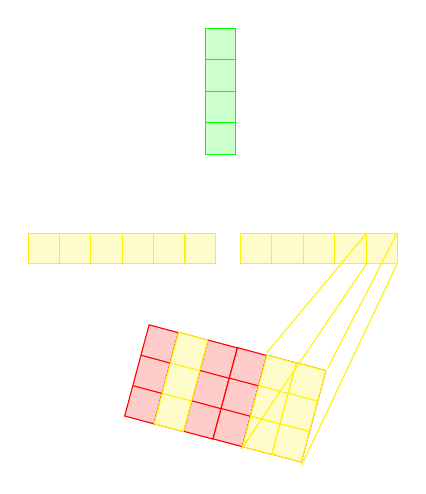
\begin{tikzpicture}[
  hid/.style 2 args={
    rectangle split,
    draw=#2,
    rectangle split parts=#1,
    fill=#2!20,
    outer sep=1mm},
  hidr/.style 2 args={
    rectangle split,
    rectangle split horizontal,
    draw=#2,
    rectangle split parts=#1,
    fill=#2!20,
    outer sep=1mm}
]

  \foreach \step in {1,...,6} {
    \node[hid={3}{red},rotate=-15,shift={(0,-.1 * \step)}] (e\step) at (.40*\step, -1) {};    
  }

  \foreach \step in {5,...,6} {
    \node[hid={3}{yellow},rotate=-15,shift={(0,-.1 * \step)}] (c\step) at (.40*\step, -1) {};    
  }
 
\node[hidr={5}{yellow}] (conv2) at (2.5,.5) {};

\draw[yellow] (1.84,-.82) -- (3.1,.69);
\draw[yellow] (1.51,-2.05) -- (3.105,.31);
\draw[yellow] (2.61,-1.02) -- (3.49,.69);
\draw[yellow] (2.28,-2.25) -- (3.495,.31);

  \foreach \step in {2,...,2} {
    \node[hid={3}{yellow},rotate=-15,shift={(0,-.1 * \step)}] (c\step) at (.40*\step, -1) {};    
  }
 
\node[hidr={6}{yellow}] (conv1) at (0,.5) {};

\node[hid={4}{green}] (s3) at (1.25, 2.5) {};
%\path[->] (concat) edge (s2);

\end{tikzpicture}


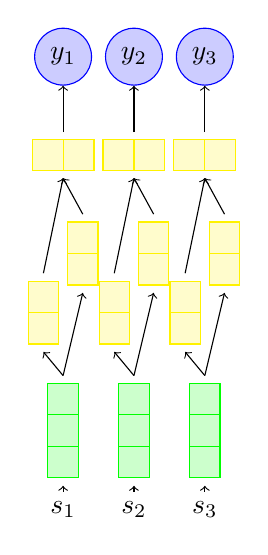
\begin{tikzpicture}[
  hid/.style 2 args={
    rectangle split,
    draw=#2,
    rectangle split parts=#1,
    fill=#2!20,
    outer sep=1mm},
  mlp/.style 2 args={
    rectangle split,
    rectangle split horizontal,
    draw=#2,
    rectangle split parts=#1,
    fill=#2!20,
    outer sep=1mm}
]

 \foreach \i [count=\step from 1] in {$s_1$, $s_2$, $s_3$}
    \node (i\step) at (.9*\step, -2) {\i};
  % draw embedding and hidden layers for text input
  \foreach \step in {1,...,3} {
    \node[hid={3}{green}] (e\step) at (.9*\step, -1) {};    
    \draw[->] (i\step.north) -> (e\step.south);
  }

  \foreach \step in {1,...,3} {
    \node[hid={2}{yellow}] (h_f_\step) at (-.25 + .9 *\step, .5) {};    
    \node[hid={2}{yellow}] (h_r_\step) at (.25 + .9 *\step, 1.25) {};    
    \draw[->] (e\step.north) -> (h_f_\step.south);
    \draw[->] (e\step.north) -> (h_r_\step.south);
    \node[mlp={2}{yellow}] (h_\step) at (.9 *\step, 2.5) {};    
    \node[circle, draw=blue, fill=blue!20] (y_\step) at (.9 *\step, 3.75) {$y_\step$};    
    \draw[->] (h_\step.north) -> (y_\step.south);
    \draw[->] (h_f_\step.north) -> (h_\step.south);
    \draw[->] (h_r_\step.north) -> (h_\step.south);
  }

\end{tikzpicture}

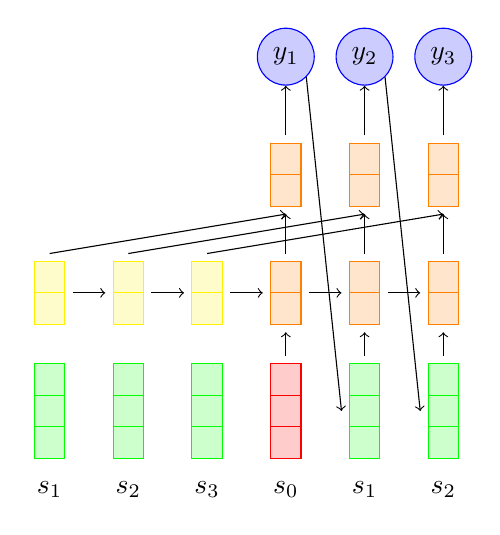
\begin{tikzpicture}[
  hid/.style 2 args={
    rectangle split,
    draw=#2,
    rectangle split parts=#1,
    fill=#2!20,
    outer sep=1mm},
  mlp/.style 2 args={
    rectangle split,
    rectangle split horizontal,
    draw=#2,
    rectangle split parts=#1,
    fill=#2!20,
    outer sep=1mm}
]

 \foreach \i [count=\step from 1] in {$s_1$, $s_2$, $s_3$, $s_0$, $s_1$, $s_2$}
    \node (i\step) at (1*\step, -2) {\i};
  % draw embedding and hidden layers for text input
  \foreach \step in {1,...,3} {
    \node[hid={3}{green}] (e\step) at (1*\step, -1) {};    
    %\draw[->] (i\step.north) -> (e\step.south);
  }
    \node[hid={3}{red}] (e4) at (1*4, -1) {};    
  \foreach \step in {5,...,6} {
    \node[hid={3}{green}] (e\step) at (1*\step, -1) {};    
    %\draw[->] (i\step.north) -> (e\step.south);
  }

  \foreach \step in {1,...,3} {
    \node[hid={2}{yellow}] (h_f_\step) at (1 *\step, .5) {};    
%    \node[hid={2}{yellow}] (h_r_\step) at (.25 + .9 *\step, 1.25) {};    
%    \draw[->] (e\step.north) -> (h_f_\step.south);
%    \draw[->] (e\step.north) -> (h_r_\step.south);
%    \node[mlp={2}{yellow}] (h_\step) at (.9 *\step, 2.5) {};    
%    \node[circle, draw=blue, fill=blue!20] (y_\step) at (.9 *\step, 3.75) {$y_\step$};    
%    \draw[->] (h_\step.north) -> (y_\step.south);
%    \draw[->] (h_f_\step.north) -> (h_\step.south);
%    \draw[->] (h_r_\step.north) -> (h_\step.south);
  }
  \foreach \step in {4,...,6} {
    \node[hid={2}{orange}] (h_f_\step) at (1 *\step, .5) {};    
    \node[hid={2}{orange}] (g_f_\step) at (1 *\step, 2) {};    
    \draw[->] (e\step.north) -> (h_f_\step.south);
    
 }
  \foreach \step in {1,...,3} {
    \node[circle, draw=blue, fill=blue!20] (y_\step) at (3 + 1 *\step, 3.5) {$y_\step$};    
 }
    \draw[->] (y_1.south east) -> (e5.west);
    \draw[->] (y_2.south east) -> (e6.west);
    \draw[->] (h_f_4.north) -> (g_f_4.south);
    \draw[->] (g_f_4.north) -> (y_1.south);
    \draw[->] (h_f_5.north) -> (g_f_5.south);
    \draw[->] (g_f_5.north) -> (y_2.south);
    \draw[->] (h_f_6.north) -> (g_f_6.south);
    \draw[->] (g_f_6.north) -> (y_3.south);
 \foreach \step/\steppp in {1/2, 2/3, 3/4, 4/5, 5/6} {
   
    \draw[->] (h_f_\step.east) -> (h_f_\steppp.west);
    %\draw[->] (h_r_\steppp.west) -> (h_r_\step.east);
  }
    \draw[->] (h_f_1.north) -> (g_f_4.south);
    \draw[->] (h_f_2.north) -> (g_f_5.south);
    \draw[->] (h_f_3.north) -> (g_f_6.south);



\end{tikzpicture}




\end{document}



%\usetikzlibrary{backgrounds}
%\usepackage{ifthen}
%% The blue print color
%\definecolor{blueprintcolor}{RGB}{20,20,100}
%
%% The shadow color
%\colorlet{shadow}{blueprintcolor!50!white}
%
%% The light color
%\colorlet{light}{white!90!blueprintcolor}
%
%% The background color
%\colorlet{background}{blueprintcolor}
%
%% The basic size of a block
%\newcommand\defaultside{0.6}
%
%% The height of a storey
%\newcommand\floorheight{0.08}
%
%% The minimum number of stories
%\newcommand\storeymin{20}
%
%% The maximum number of stories
%\newcommand\storeymax{40}
%
%% The width of a window
%\newcommand\window{0.05}
%
%% The angles of x,y-axes
%\newcommand\xaxis{210}
%\newcommand\yaxis{-30}
%
%% Facade style random list
%\pgfmathdeclarerandomlist{facade}{{\hlines}{\vlines}{\grid}{\grid}{\grid}}
%
%% Vertical thickness
%\newcommand\vthickness{thin}
%
%% Horizontal thickness
%\newcommand\hthickness{thin}
%
%% Selects at random the thickness of the horizontal lines
%\newcommand\setvthickness{
%  \pgfmathrandominteger{\alea}{0}{3}
%  \ifthenelse{\alea=0}{\renewcommand\vthickness{thick}}{}
%  \ifthenelse{\alea=1}{\renewcommand\vthickness{thin}}{}
%  \ifthenelse{\alea=2}{\renewcommand\vthickness{very thin}}{}
%  \ifthenelse{\alea=3}{\renewcommand\vthickness{ultra thin}}{}
%}
%
%% Selects at random the thickness of the vertical lines
%\newcommand\seththickness{
%  \pgfmathrandominteger{\alea}{0}{3}
%  \ifthenelse{\alea=0}{\renewcommand\hthickness{thick}}{}
%  \ifthenelse{\alea=1}{\renewcommand\hthickness{thin}}{}
%  \ifthenelse{\alea=2}{\renewcommand\hthickness{very thin}}{}
%  \ifthenelse{\alea=3}{\renewcommand\hthickness{ultra thin}}{}
%}
%
%% Draws vertical lines on each side of the block
%\newcommand\vlines[2]{
%  \pgfmathsetmacro\size{#1 * \floorheight}
%  \pgfmathsetmacro\max{#2/\window}
%  \foreach \col in {1,...,\max}
%  {
%    \pgfmathsetmacro\xx{-\col * \window}    
%    \draw[\vthickness,draw=shadow, shift={(\yaxis:\xx)}] (0,0)--(0,\size);
%    \draw[\vthickness,draw=light, shift={(\xaxis:\xx)}] (0,0)--(0,\size);
%  }  
%}
%
%% Draws horizontal lines on each side of the block
%\newcommand\hlines[2]{
%  \foreach \floor in {0,...,#1}
%  {
%    \pgfmathsetmacro\z{\floor * \floorheight}    
%    \draw[\hthickness,draw=shadow, shift={(90:\z)}] (150:#2)--(0,0);
%    \draw[\hthickness,draw=light, shift={(90:\z)}] (0,0) -- (30:#2);
%  }
%}
%
%% Draws horizontal and vertical lines on each side of the block
%\newcommand\grid[2]{
%  \vlines{#1}{#2}
%  \hlines{#1}  {#2}
%}
%
%% Draws a block at the specified position
%\newcommand\block[2]{
%  % Computes the height of the block
%  \pgfmathsetmacro\height{#2 * \floorheight}
%    
%  % Erases the background
%  \fill[fill=background]
%    (0,0) -- (150:#1) -- ++(0,\height) -- (0,\height) -- (0,0);
%  \fill[fill=background]
%    (0,0) -- (30:#1) -- ++(0,\height) -- (0,\height) -- (0,0);
%  
%  % Draws the facades
%  \facade{\stories}{#1}
%  
%  % Frames the facades
%  \draw[draw=shadow] (0,0) -- (150:#1) -- ++(0,\height) -- (0,\height) -- (0,0);
%  \draw[draw=light] (0,0) -- (30:#1) -- ++(0,\height) -- (0,\height) -- (0,0);
%  
%  % Draws the terrace
%  \fill[fill=background, draw=light,shift={(90:\height)}]
%    (0,0) -- (30:#1) -- (0,#1) --(150:#1)--(0,0);
%
%  %
%  \pgfmathrandominteger{\alea}{0}{3}
%  \ifthenelse{\alea=0}{
%  % Sometimes, adds more stores (= skyscraper)
%    \begin{scope}[shift={(0,\height)},shift={(0,0.05)}]
%      \pgfmathsetmacro\pside{#1-0.1}
%      \pgfmathrandominteger{\stories}{2}{\storeymax}
%      \block{\pside}{\stories}
%    \end{scope}  
%  }{}
%  
%  \ifthenelse{\alea=1}{
%  % Sometimes, draws a pyramid roof
%  \pyramid{\height}{#1}  
%  }{}
%}
%
%% Draws a basic block
%\newcommand\basicblock[3]{
%  % Selects a random facade style
%  \pgfmathrandomitem{\facade}{facade}
%  \setvthickness{}
%  \seththickness{}
%  
%  % Selects a random number of stores
%  \pgfmathrandominteger{\stories}{\storeymin}{\storeymax}
%  
%  \begin{scope}[shift={(\xaxis:#1)},shift={(\yaxis:#2)}]
%  \block{#3}{\stories}
%  \end{scope}
%}
%
%% Draws a pyramid roof
%\newcommand\pyramid[2]{
%  % Computes the side of the pyramid
%  \pgfmathsetmacro\pside{#2-0.1}
%
%  % Selects the height of the pyramid at random
%  \pgfmathparse{random()}
%  \pgfmathsetmacro\top{0.5+\pgfmathresult/3}
%
%  % Draws the pyramid
%  \begin{scope}[fill=background, draw=light,shift={(90:#1)},shift={(90:0.05)}]
%    \fill[draw=light] (0,0) -- (30:\pside) -- (0,\top) -- (150:\pside)--(0,0);
%    \draw (0,0) -- (0,\top);
%  \end{scope}
%}
%
%% Draws a random city of the specified dimensions
%\newcommand\city[2]{
%  \foreach \x in {1,...,#1}
%    \foreach \y in {1,...,#2}
%      {\basicblock{\x}{\y}{\defaultside}}
%}
%
%\begin{document} 
%% Draws a hundred blocks random city
%\begin{tikzpicture}[show background rectangle,
%  background rectangle/.style={fill=background}]
%    \city{10}{10}
%\end{tikzpicture}
%\end{document}
%
